\documentclass[a4paper,11pt]{article}

\usepackage[swedish]{babel}
\usepackage[T1]{fontenc}
\usepackage[utf8]{inputenc}
\usepackage{hyperref}
\usepackage{listings}
\usepackage{xcolor}
\usepackage{graphicx}
\usepackage{float}

\lstset{
  basicstyle=\ttfamily\small,
  backgroundcolor=\color{gray!10},
  frame=single,
  breaklines=true
}

\begin{document} 

\section*{Användarmanual}
Vår applikation är en webbaserad plattform som möjliggör effektiv hantering av tävlande och stationer i en tävling.

Den går att installera på en lokal server eller i molnet, och är tillgänglig via en webbläsare.

I den kan du registrera stationer, tävlande och stopptider, samt visa resultat i realtid. Du kan även ha flera olika tävlingar samtidigt, där varje tävling har sina egna stationer och tävlande.\\

Denna användarmanual är avsedd för administratörer och användare av vår applikation. Den innehåller instruktioner för att navigera och använda de olika funktionerna i systemet.\\
Applikationen är utformad för att vara användarvänlig och intuitiv, med minimal grafisk design för att fokusera på funktionalitet och användarupplevelse. 

\section{Grafisk navigering}

I frontenden möts användaren av en startsida. På samtliga sidor finns en knapp för att aktivera \textbf{Dark Mode}.  

\begin{figure}[H]
  \centering
  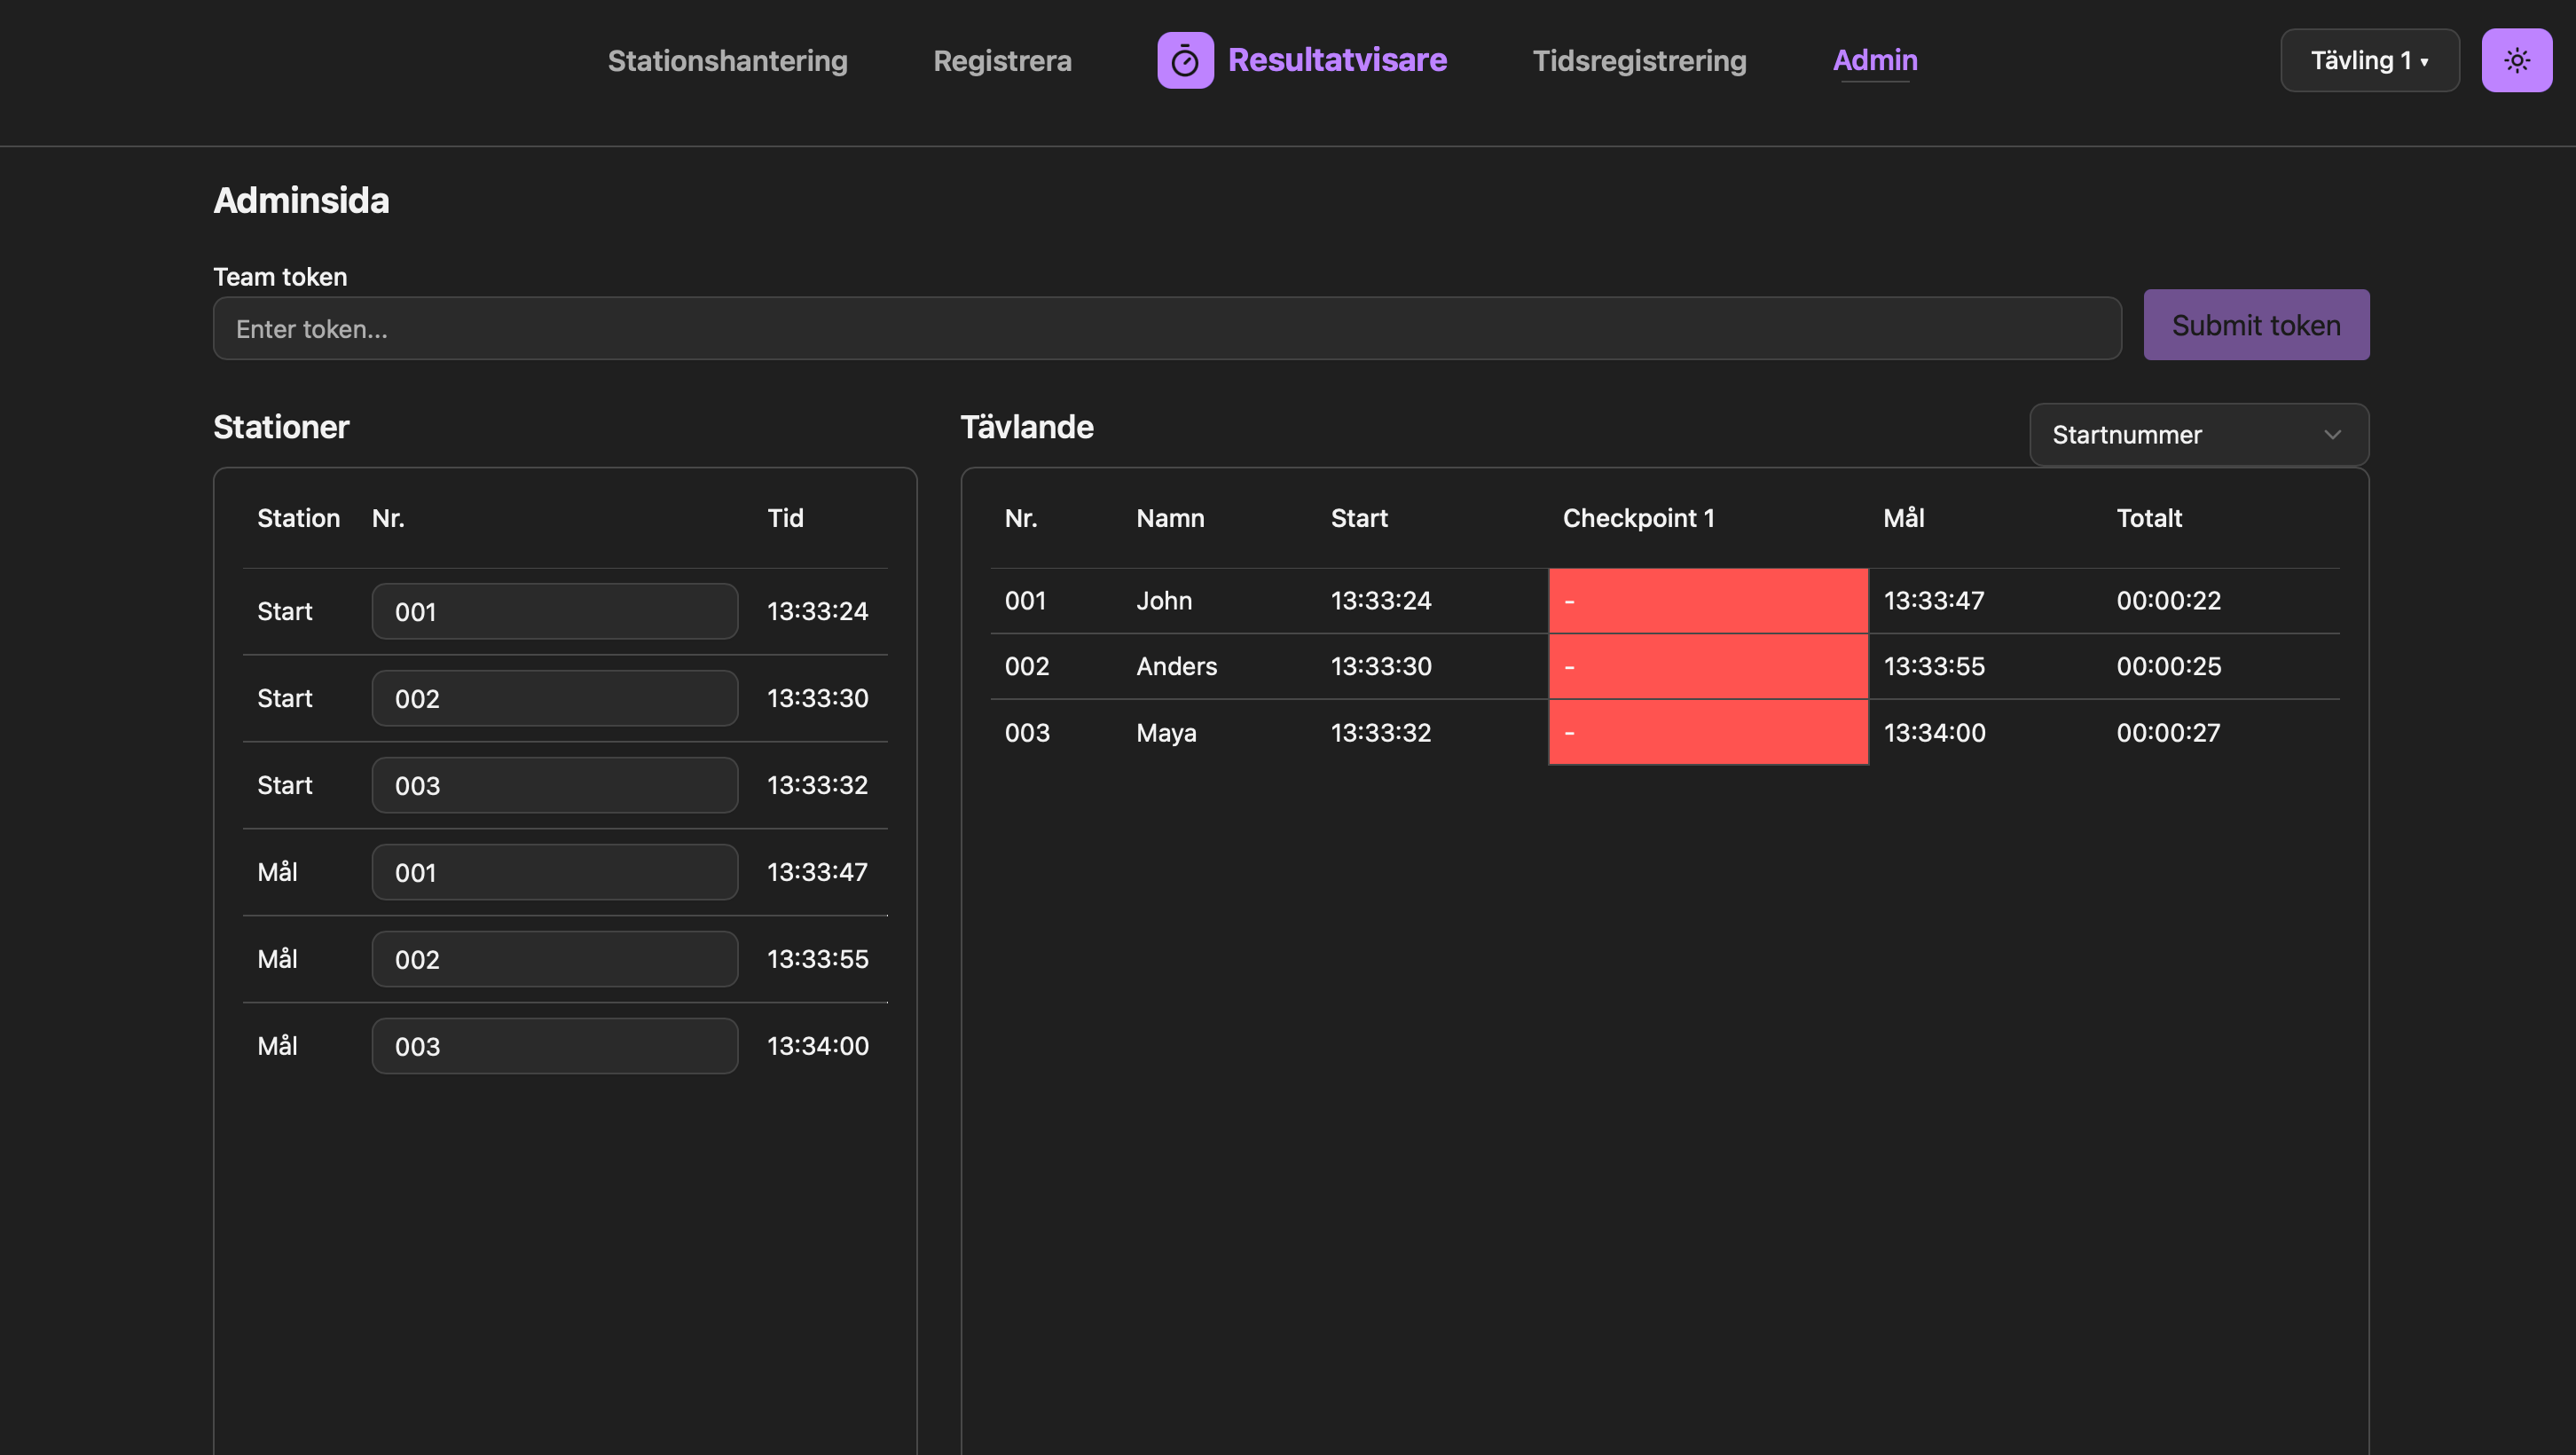
\includegraphics[width=0.7\textwidth]{Screenshots till användarmanual/Dark-mode2.png}
  \caption{Dark mode}
  \label{fig:Dark mode}
\end{figure}

Frontend innehåller följande sidor:

\subsection{Stationshantering}
Innehåller två inmatningsfält och en registreringsknapp där man kan registrera stationer genom att skriva in stationsnamn och ordning.  
Under formuläret visas en tabell med de registrerade stationerna. På varje stationsrad finns även en radera-funktion som tar bort stationen. 

\begin{figure}[H]
  \centering
  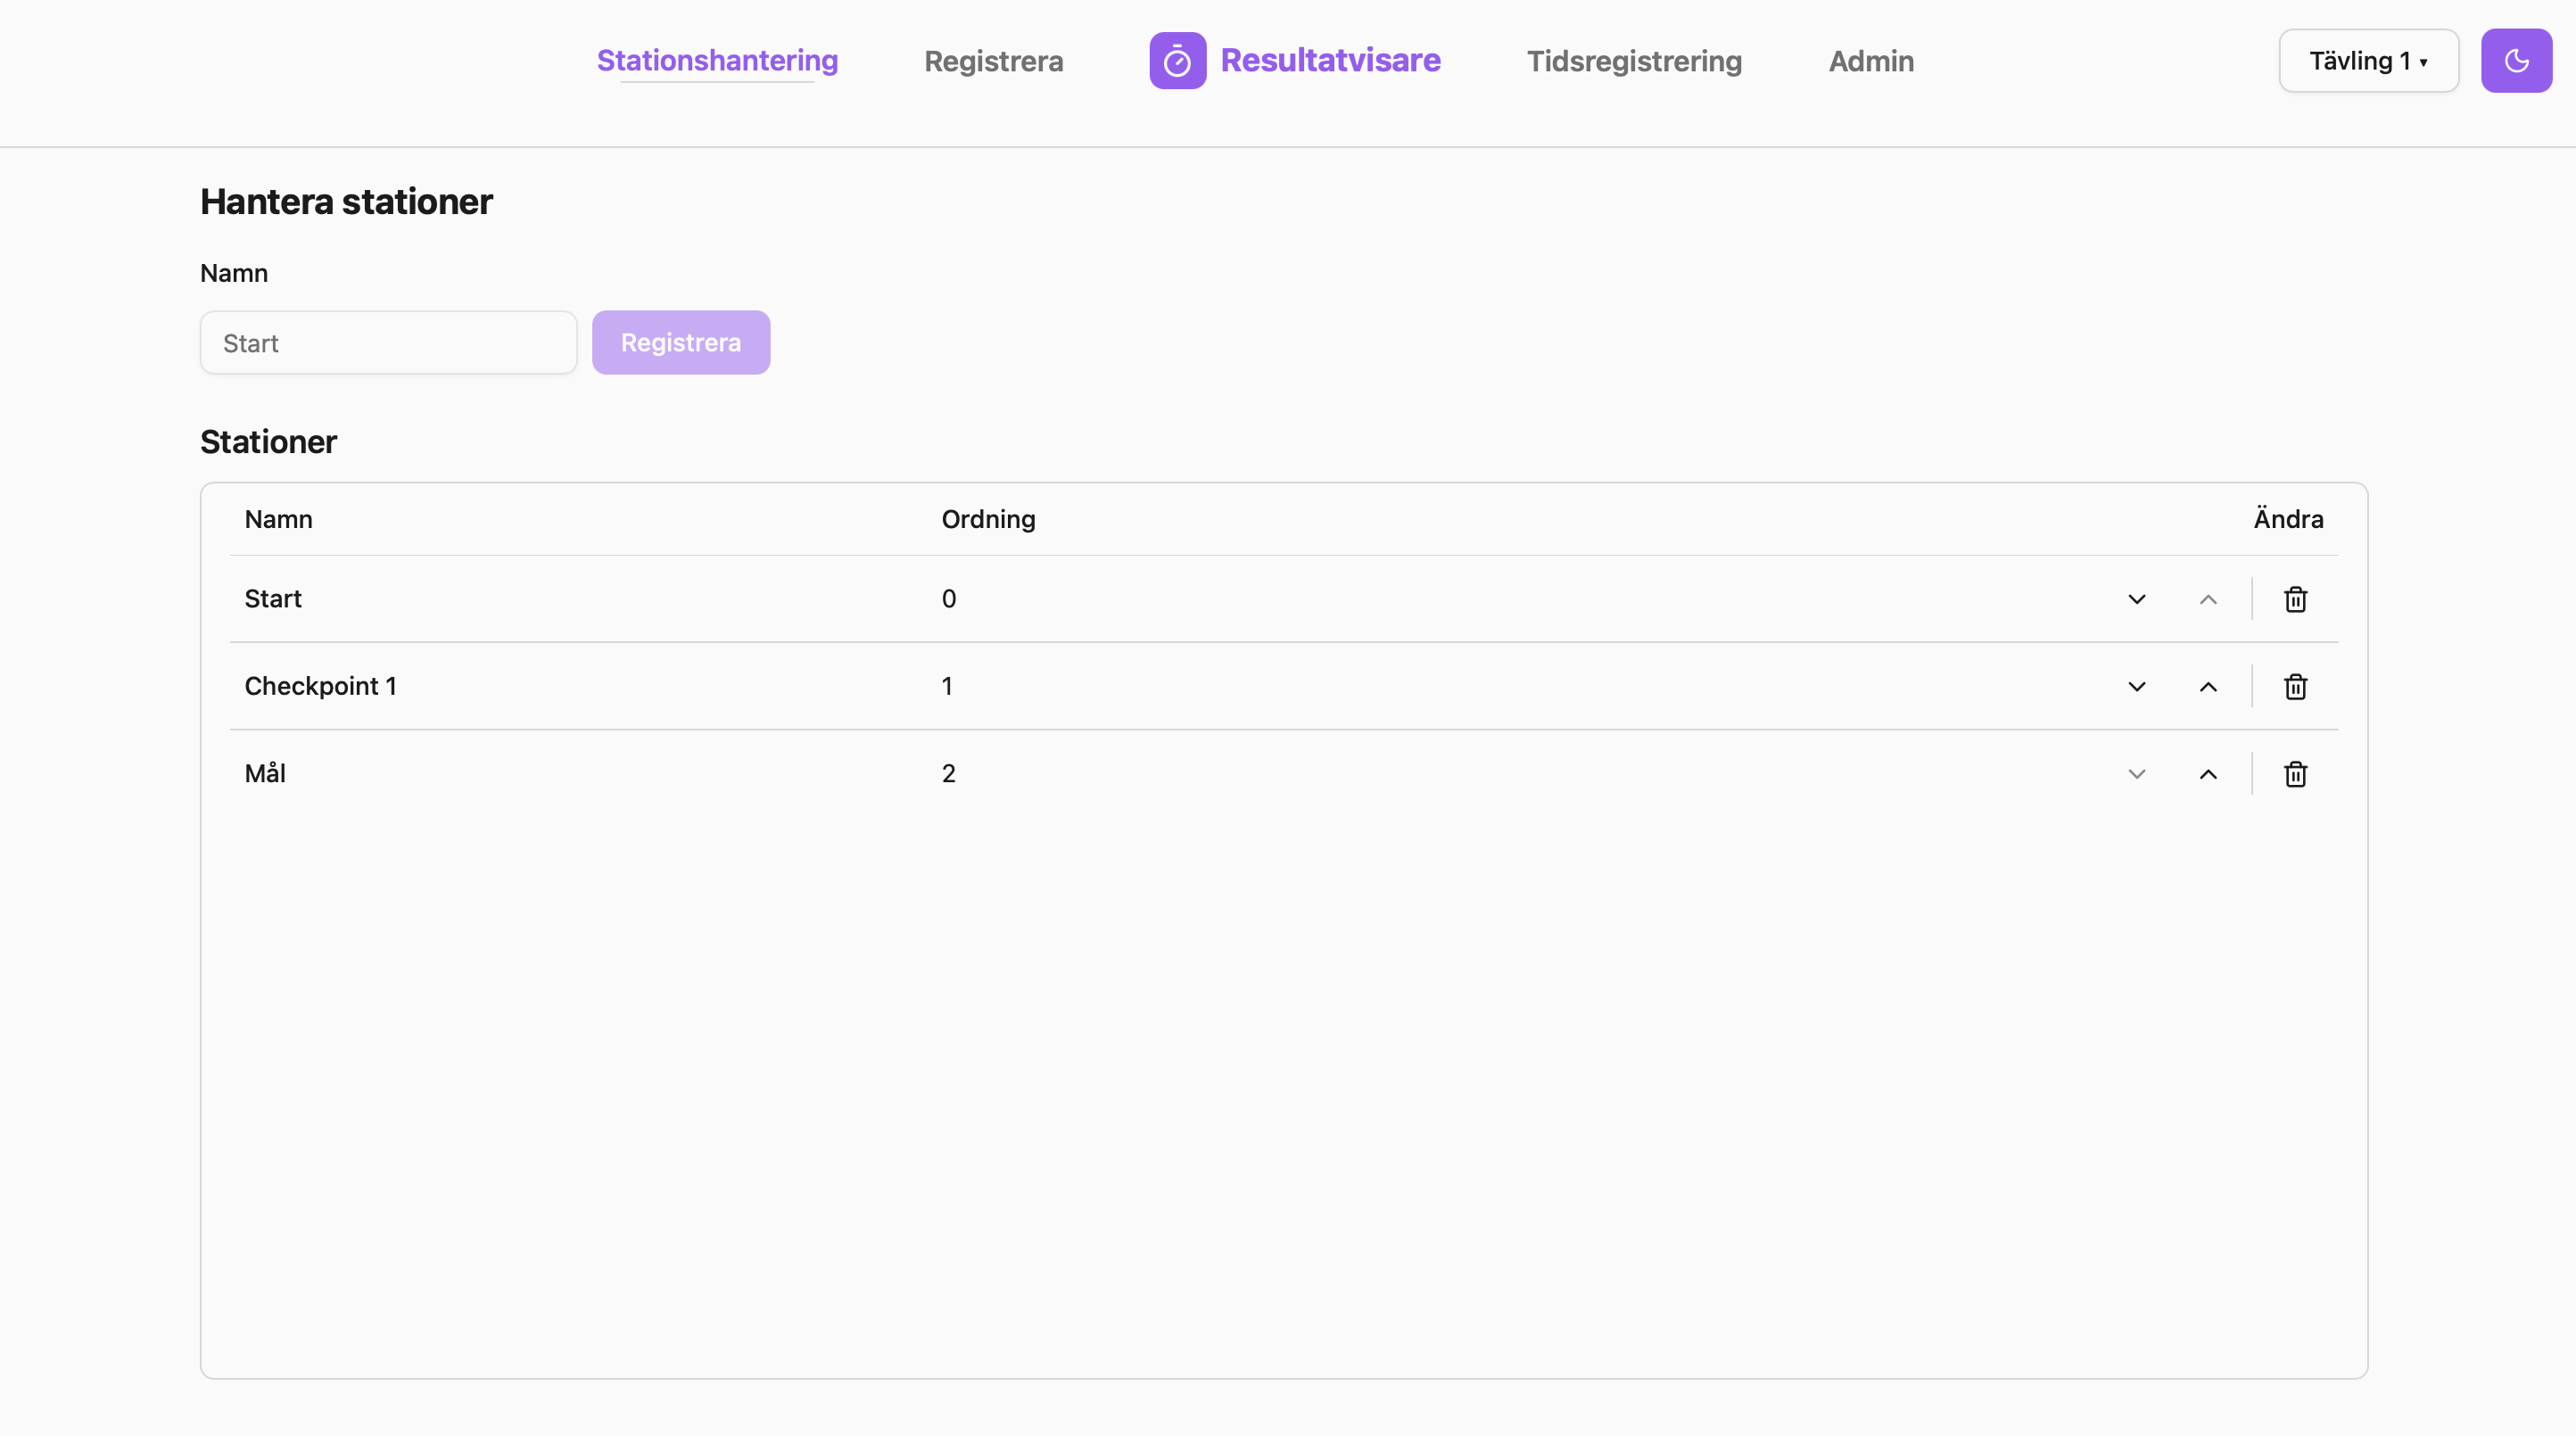
\includegraphics[width=0.7\textwidth]{Screenshots till användarmanual/Stationshanterare2.png}
  \caption{Stationshanteringssida}
  \label{fig:Stationshantering}
\end{figure}

\subsection{Registrera}

Innehåller ett inmatningsfält där man kan registrera startnummer och namn på en tävlande.  
Under formuläret visas en tabell med de registrerade tävlande. Det finns även funktioner för att redigera och radera tävlande. Under redigera kan både startnummer och namn ändras. 

\begin{figure}[H]
  \centering
  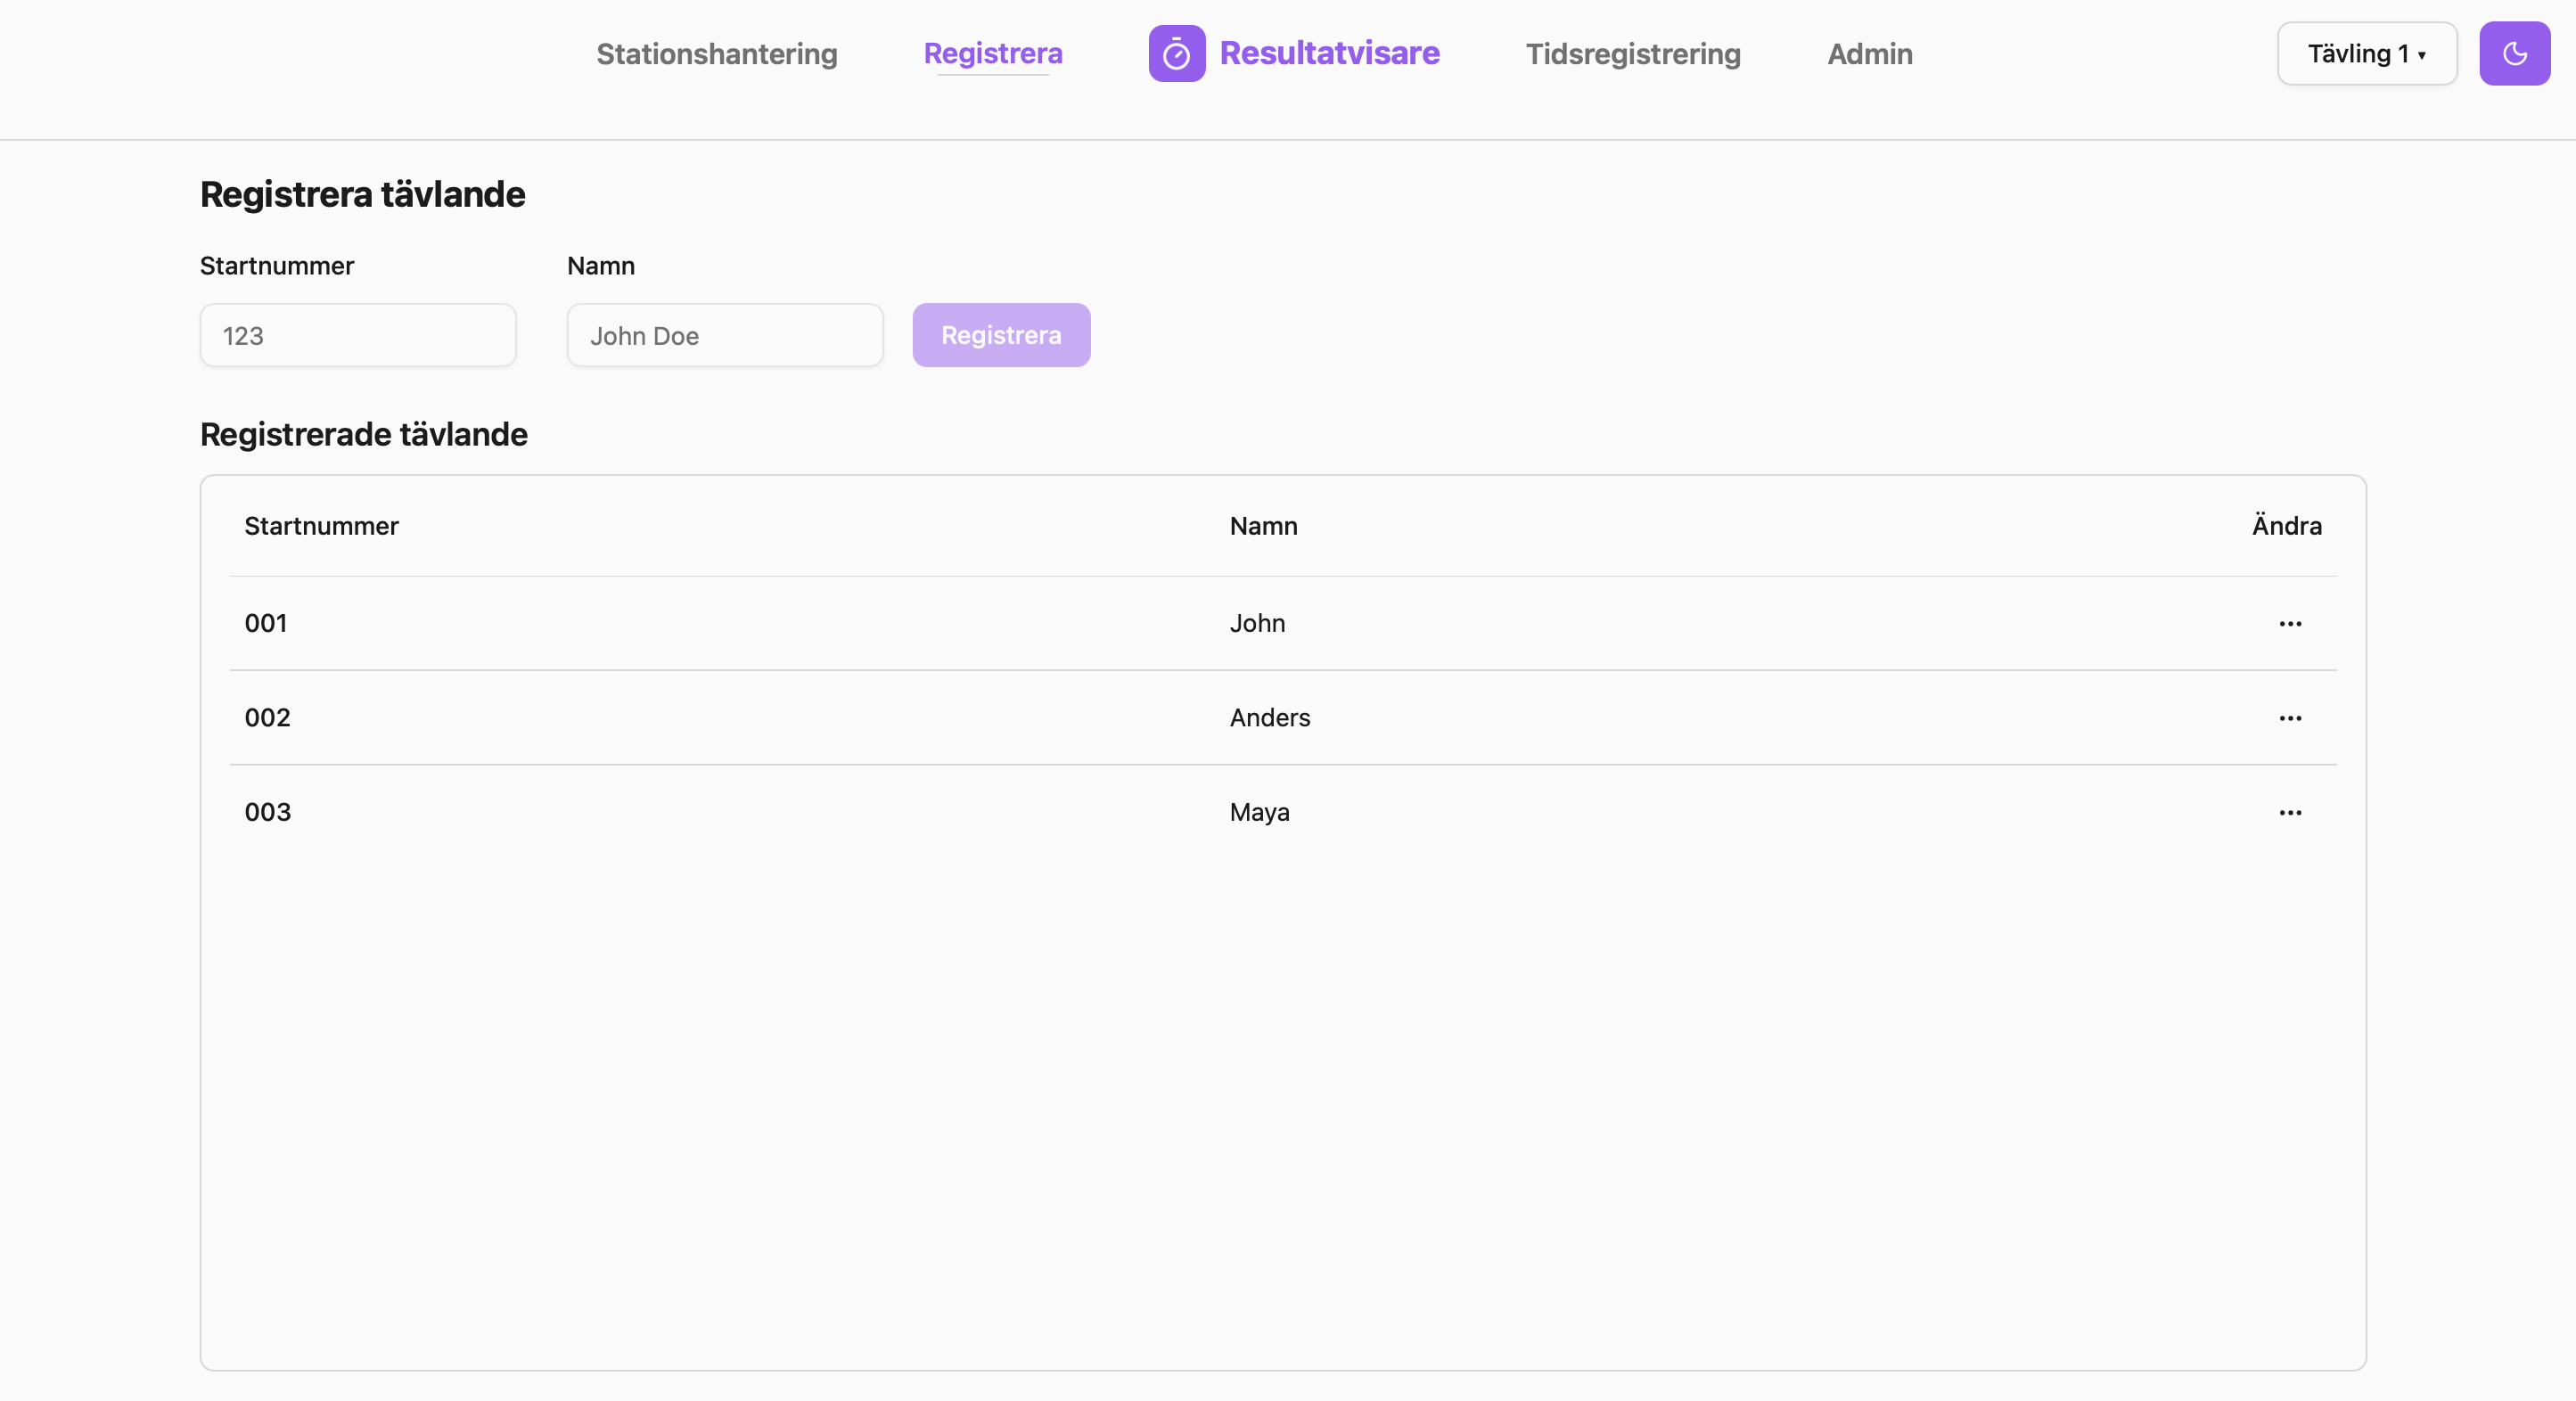
\includegraphics[width=0.7\textwidth]{Screenshots till användarmanual/Registrera2.png}
  \caption{Registreringssida}
  \label{fig:Registreringssida}
\end{figure}

\subsection{Startsidan}
Innehåller en resultatvisare som har en lista på alla tävlande med rang, startnummer, namn och totaltid, sorterad på totaltid.

\begin{figure}[H]
  \centering
  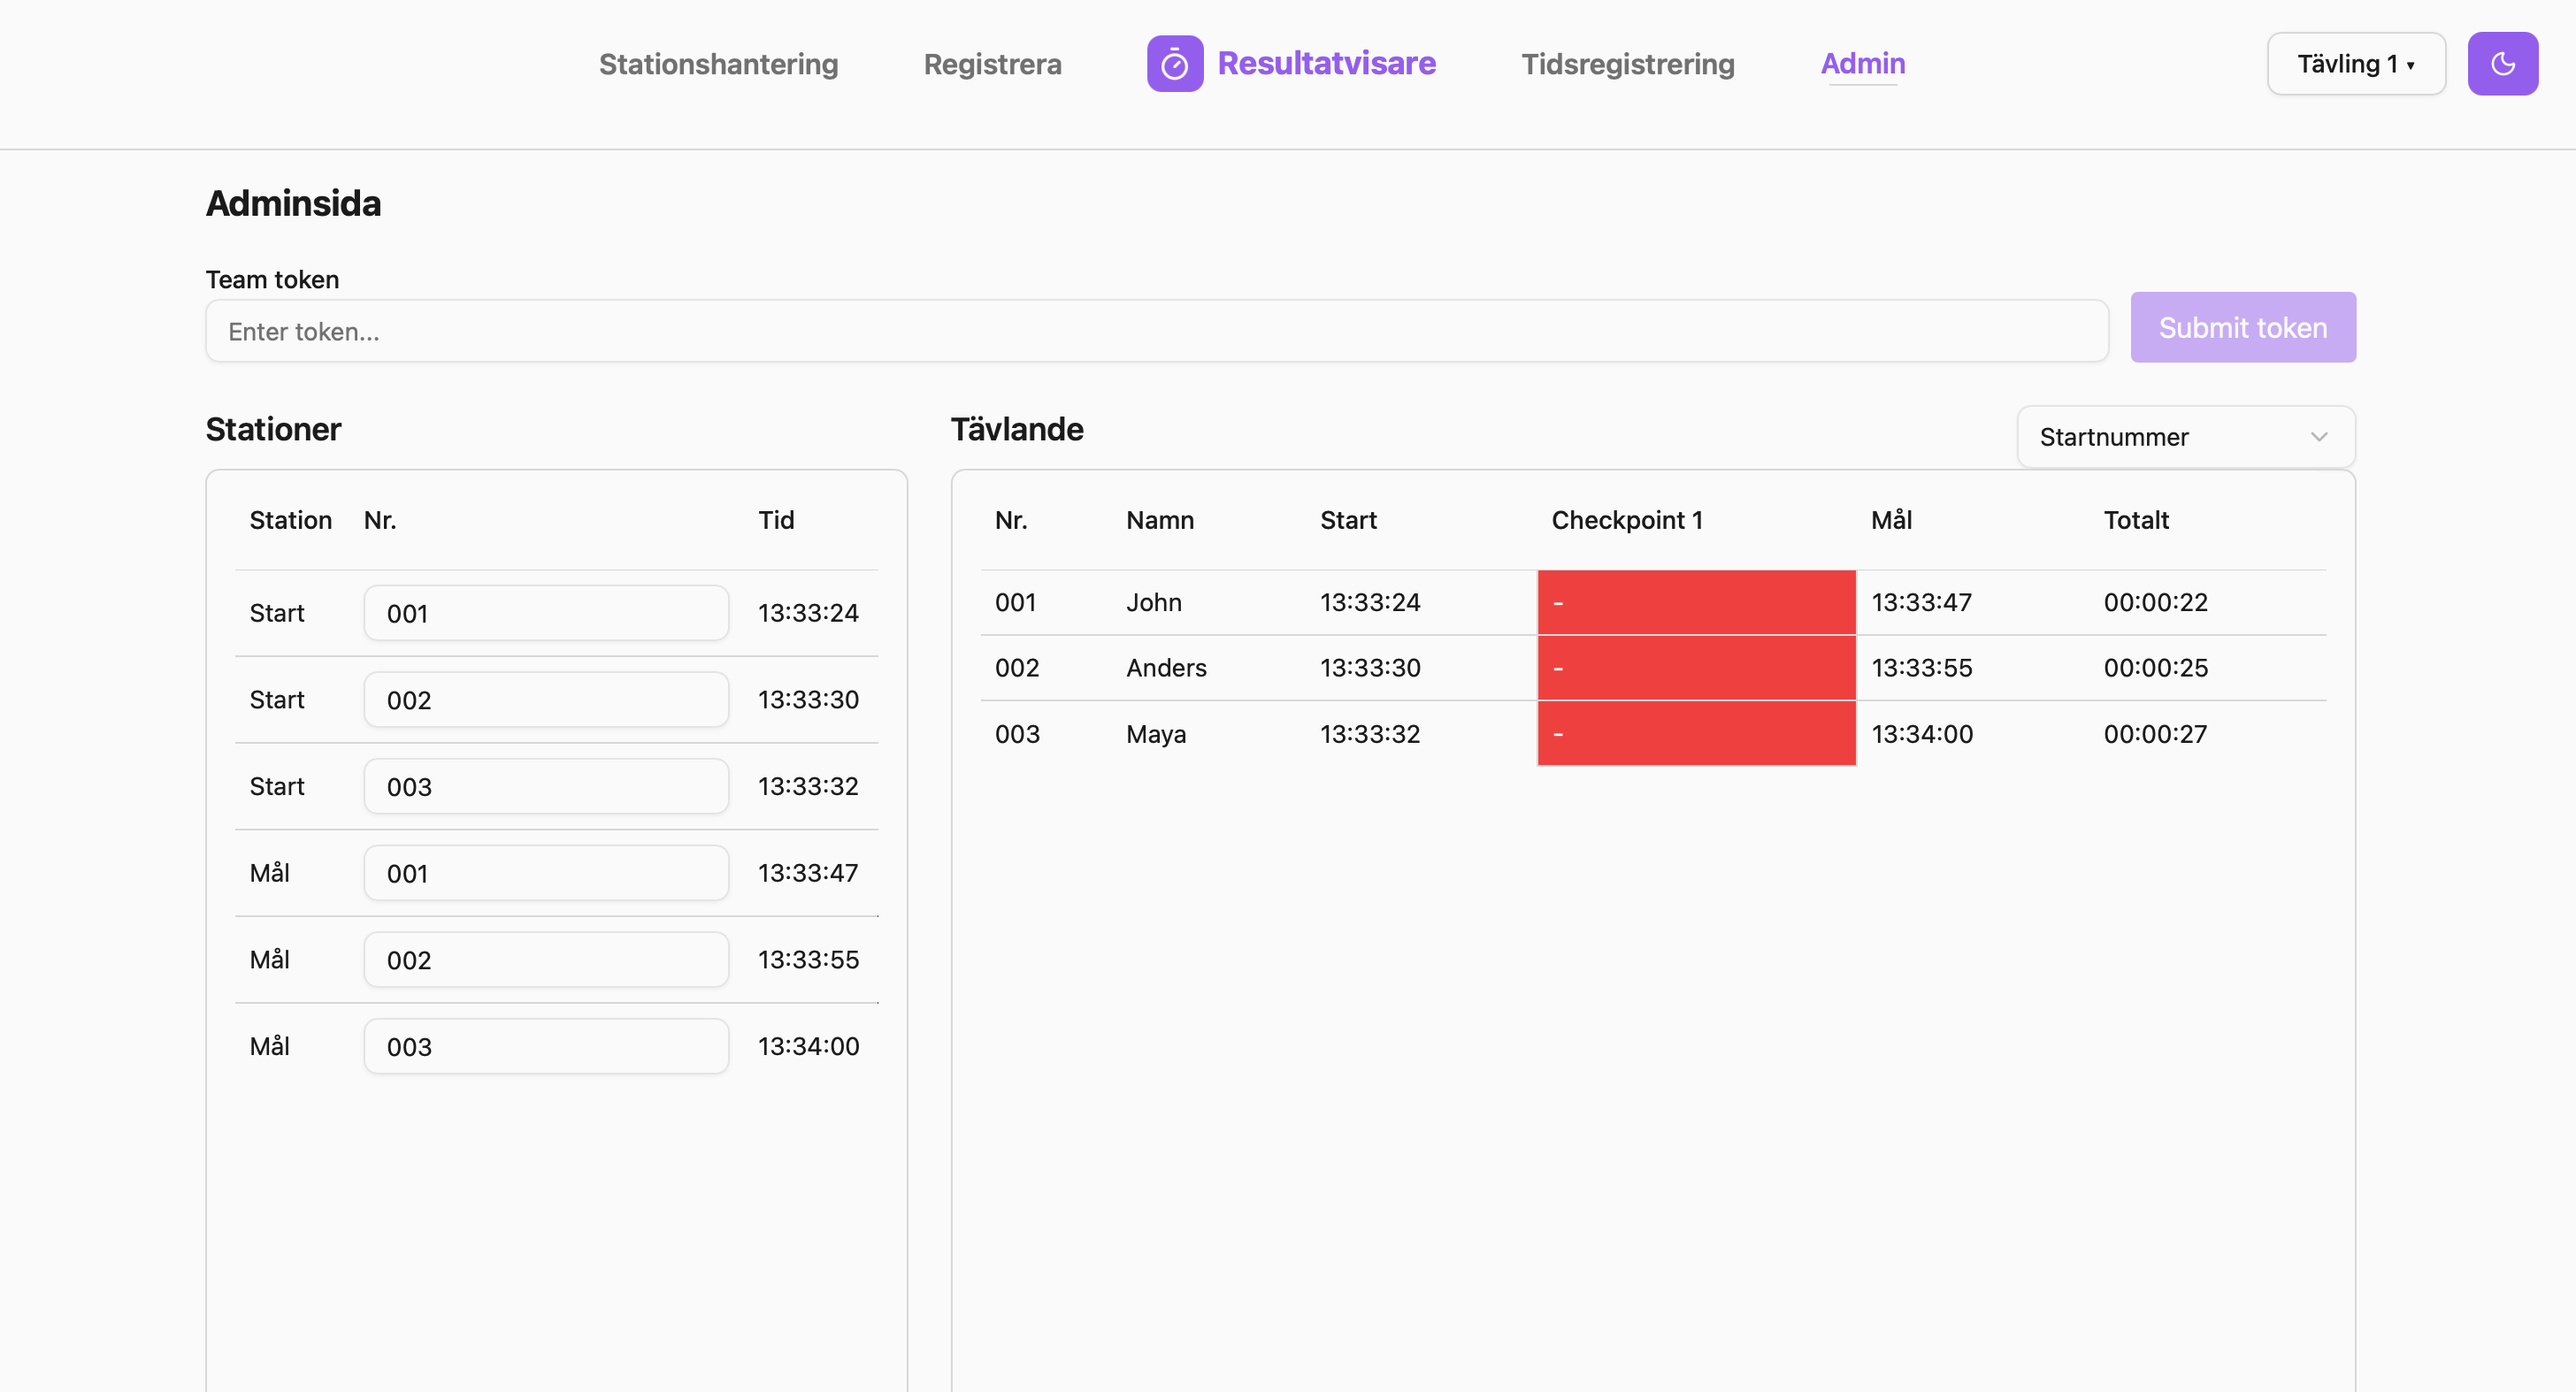
\includegraphics[width=0.7\textwidth]{Screenshots till användarmanual/Resultatvisare2.png}
  \caption{Startsida med resultatvisare}
  \label{fig:Resultatvisare}
\end{figure}

\subsection{Stopptid}
Innehåller två dropdown-menyer och ett sökfält där man väljer bland stationer och registrerade tävlande.  

Det finns två knappar:
\begin{enumerate}
  \item Registrerar stopptiden
  \item Uppdaterar listan
\end{enumerate}

Under dessa visas 2 tabeller: en tabell över registrerade tävlande med deras startnummer. Den andra tabellen visar senaste registreringar av stopptid med tiden registreringen skedde, startnummer och namn på tävlande och stationen som registreringen skedde på.

\begin{figure}[H]
  \centering
  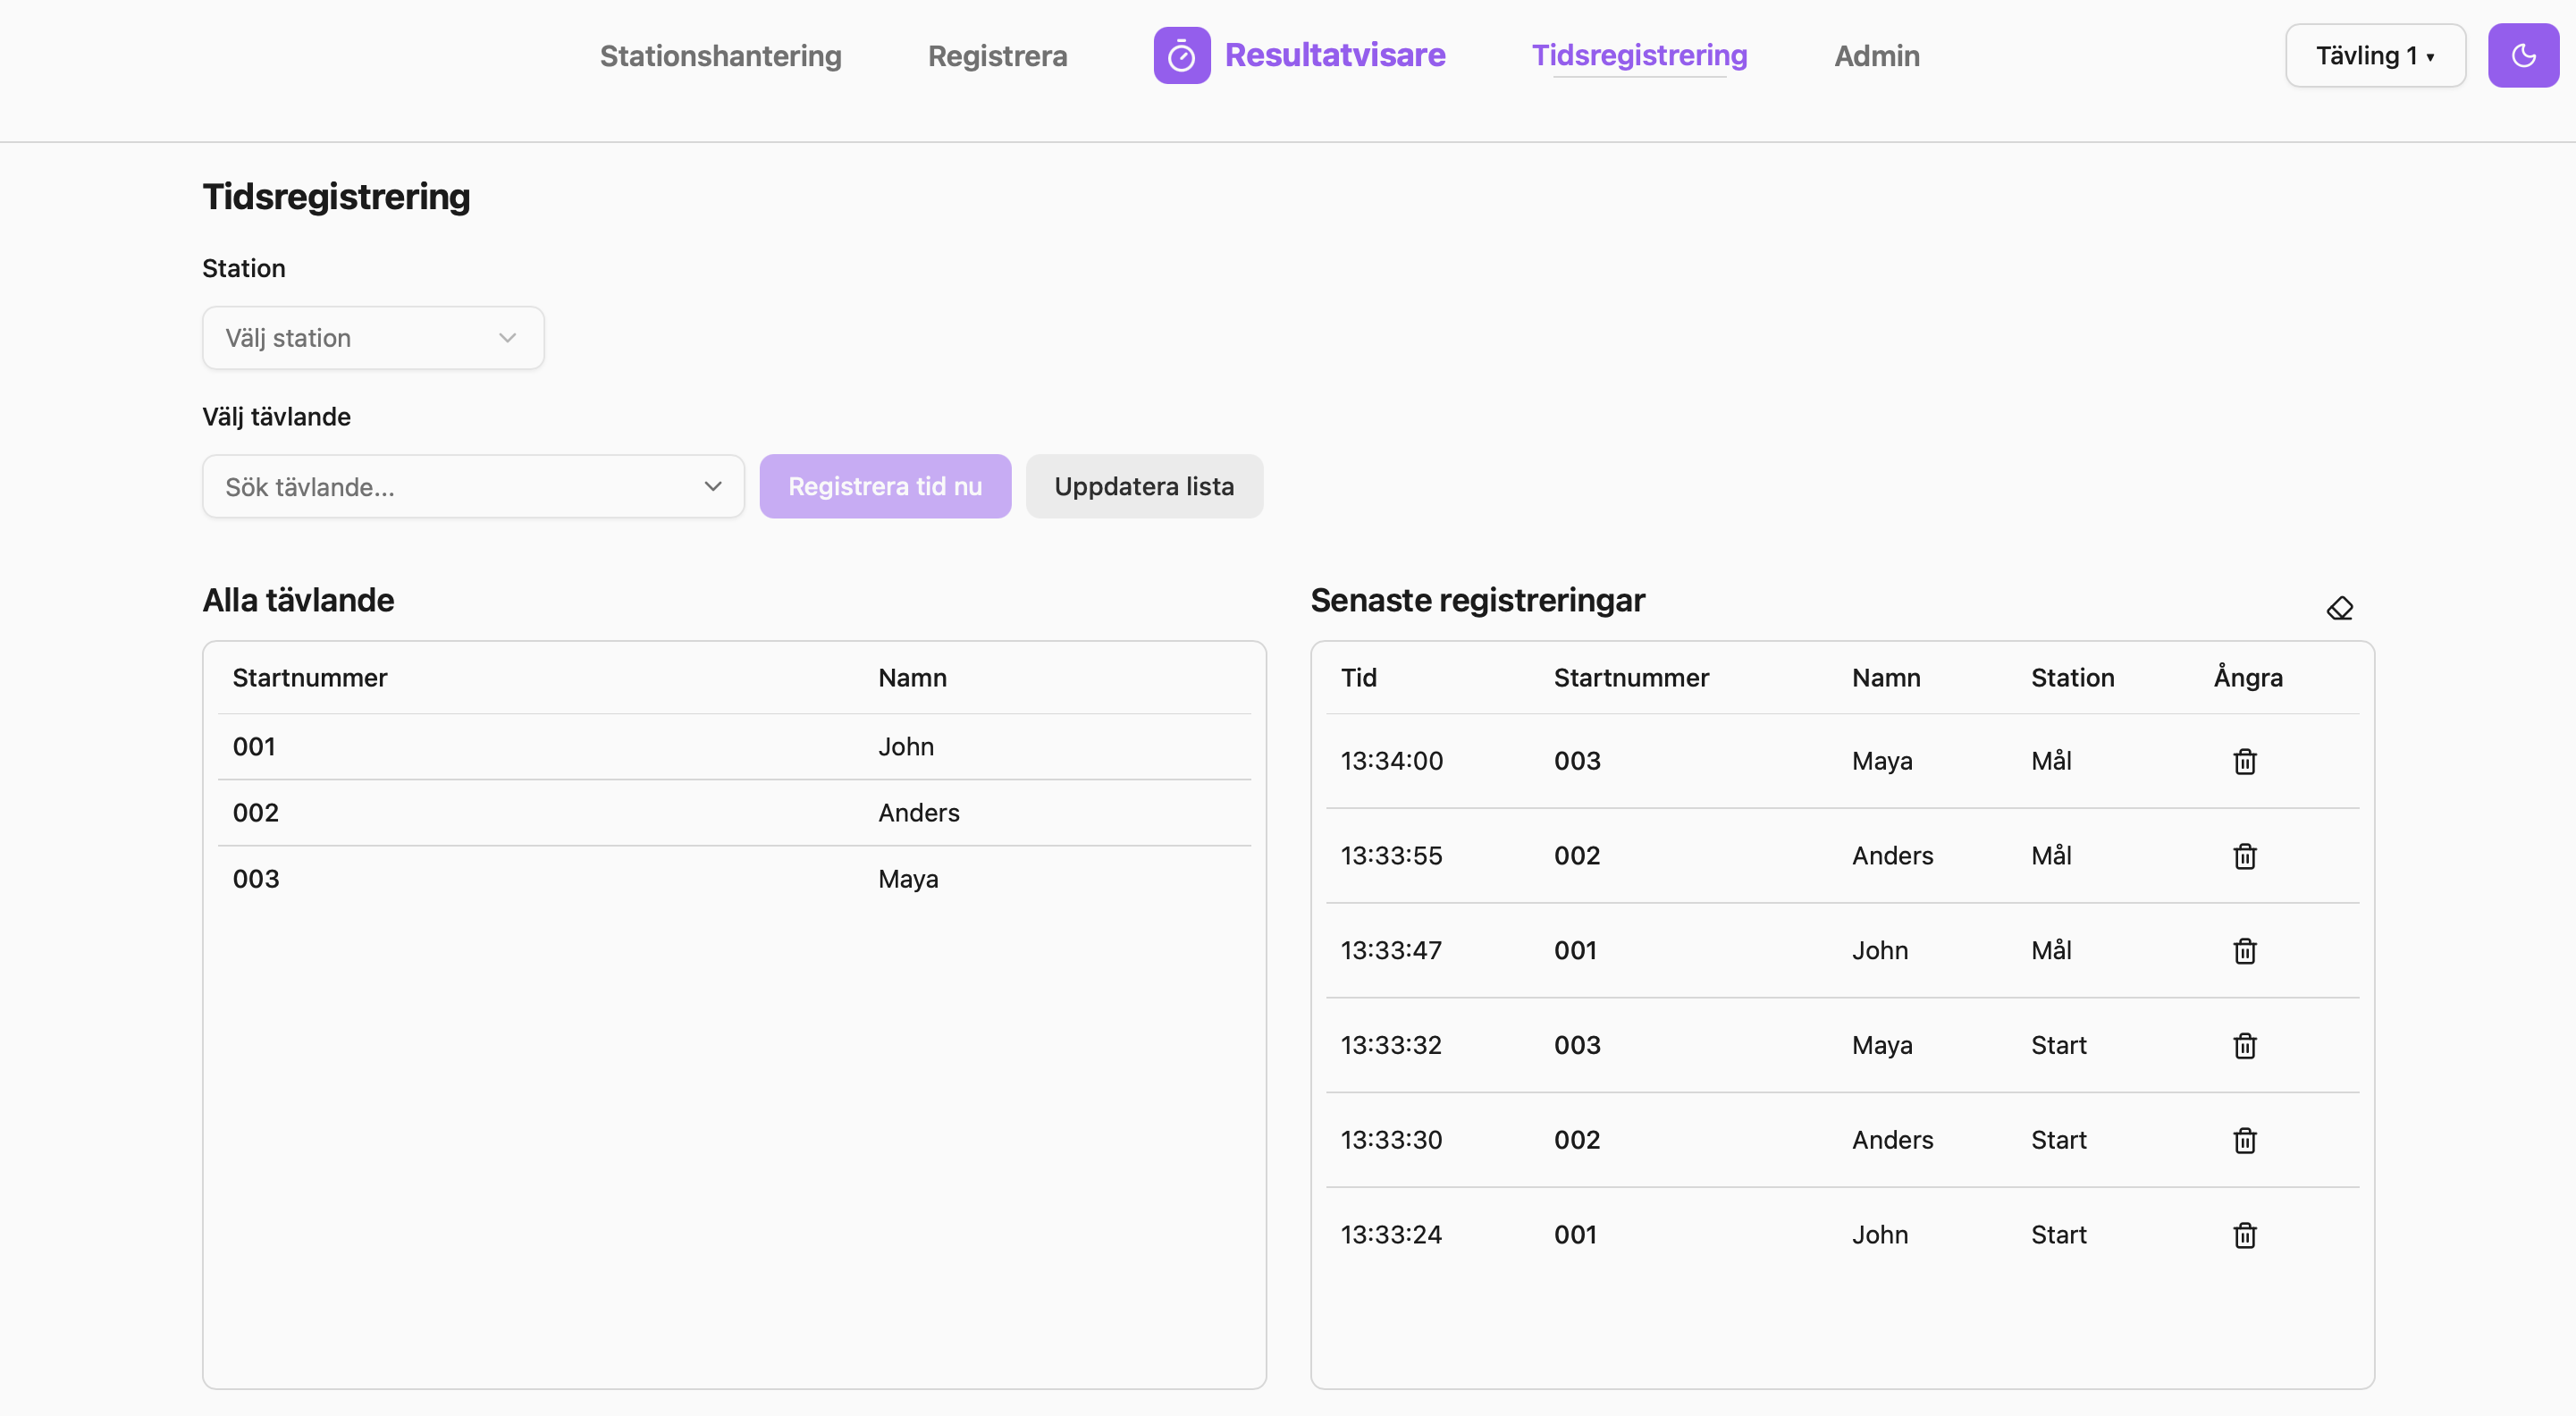
\includegraphics[width=0.7\textwidth]{Screenshots till användarmanual/Tidsregstrering2.png}
  \caption{Tidsregistrering}
  \label{fig:Tidsregistrering}
\end{figure}

\subsection{Admin}
En kontinuerligt uppdaterad vy som visar registrerade tävlande med rang, startnummer, namn och total tid.

Högst upp presenteras ett fält för att skriva in token samt en knapp att skicka resultat till servern


Här presenteras all information om de tävlande i två tabeller:
\begin{itemize}
  \item Station, startnummer och tid
  \item Startnummer, namn, starttid, måltid och totalt resultat (sorterad på startnummer)
\end{itemize}

Röda rutor indikerar felaktig registrering.

\begin{figure}[H]
  \centering
  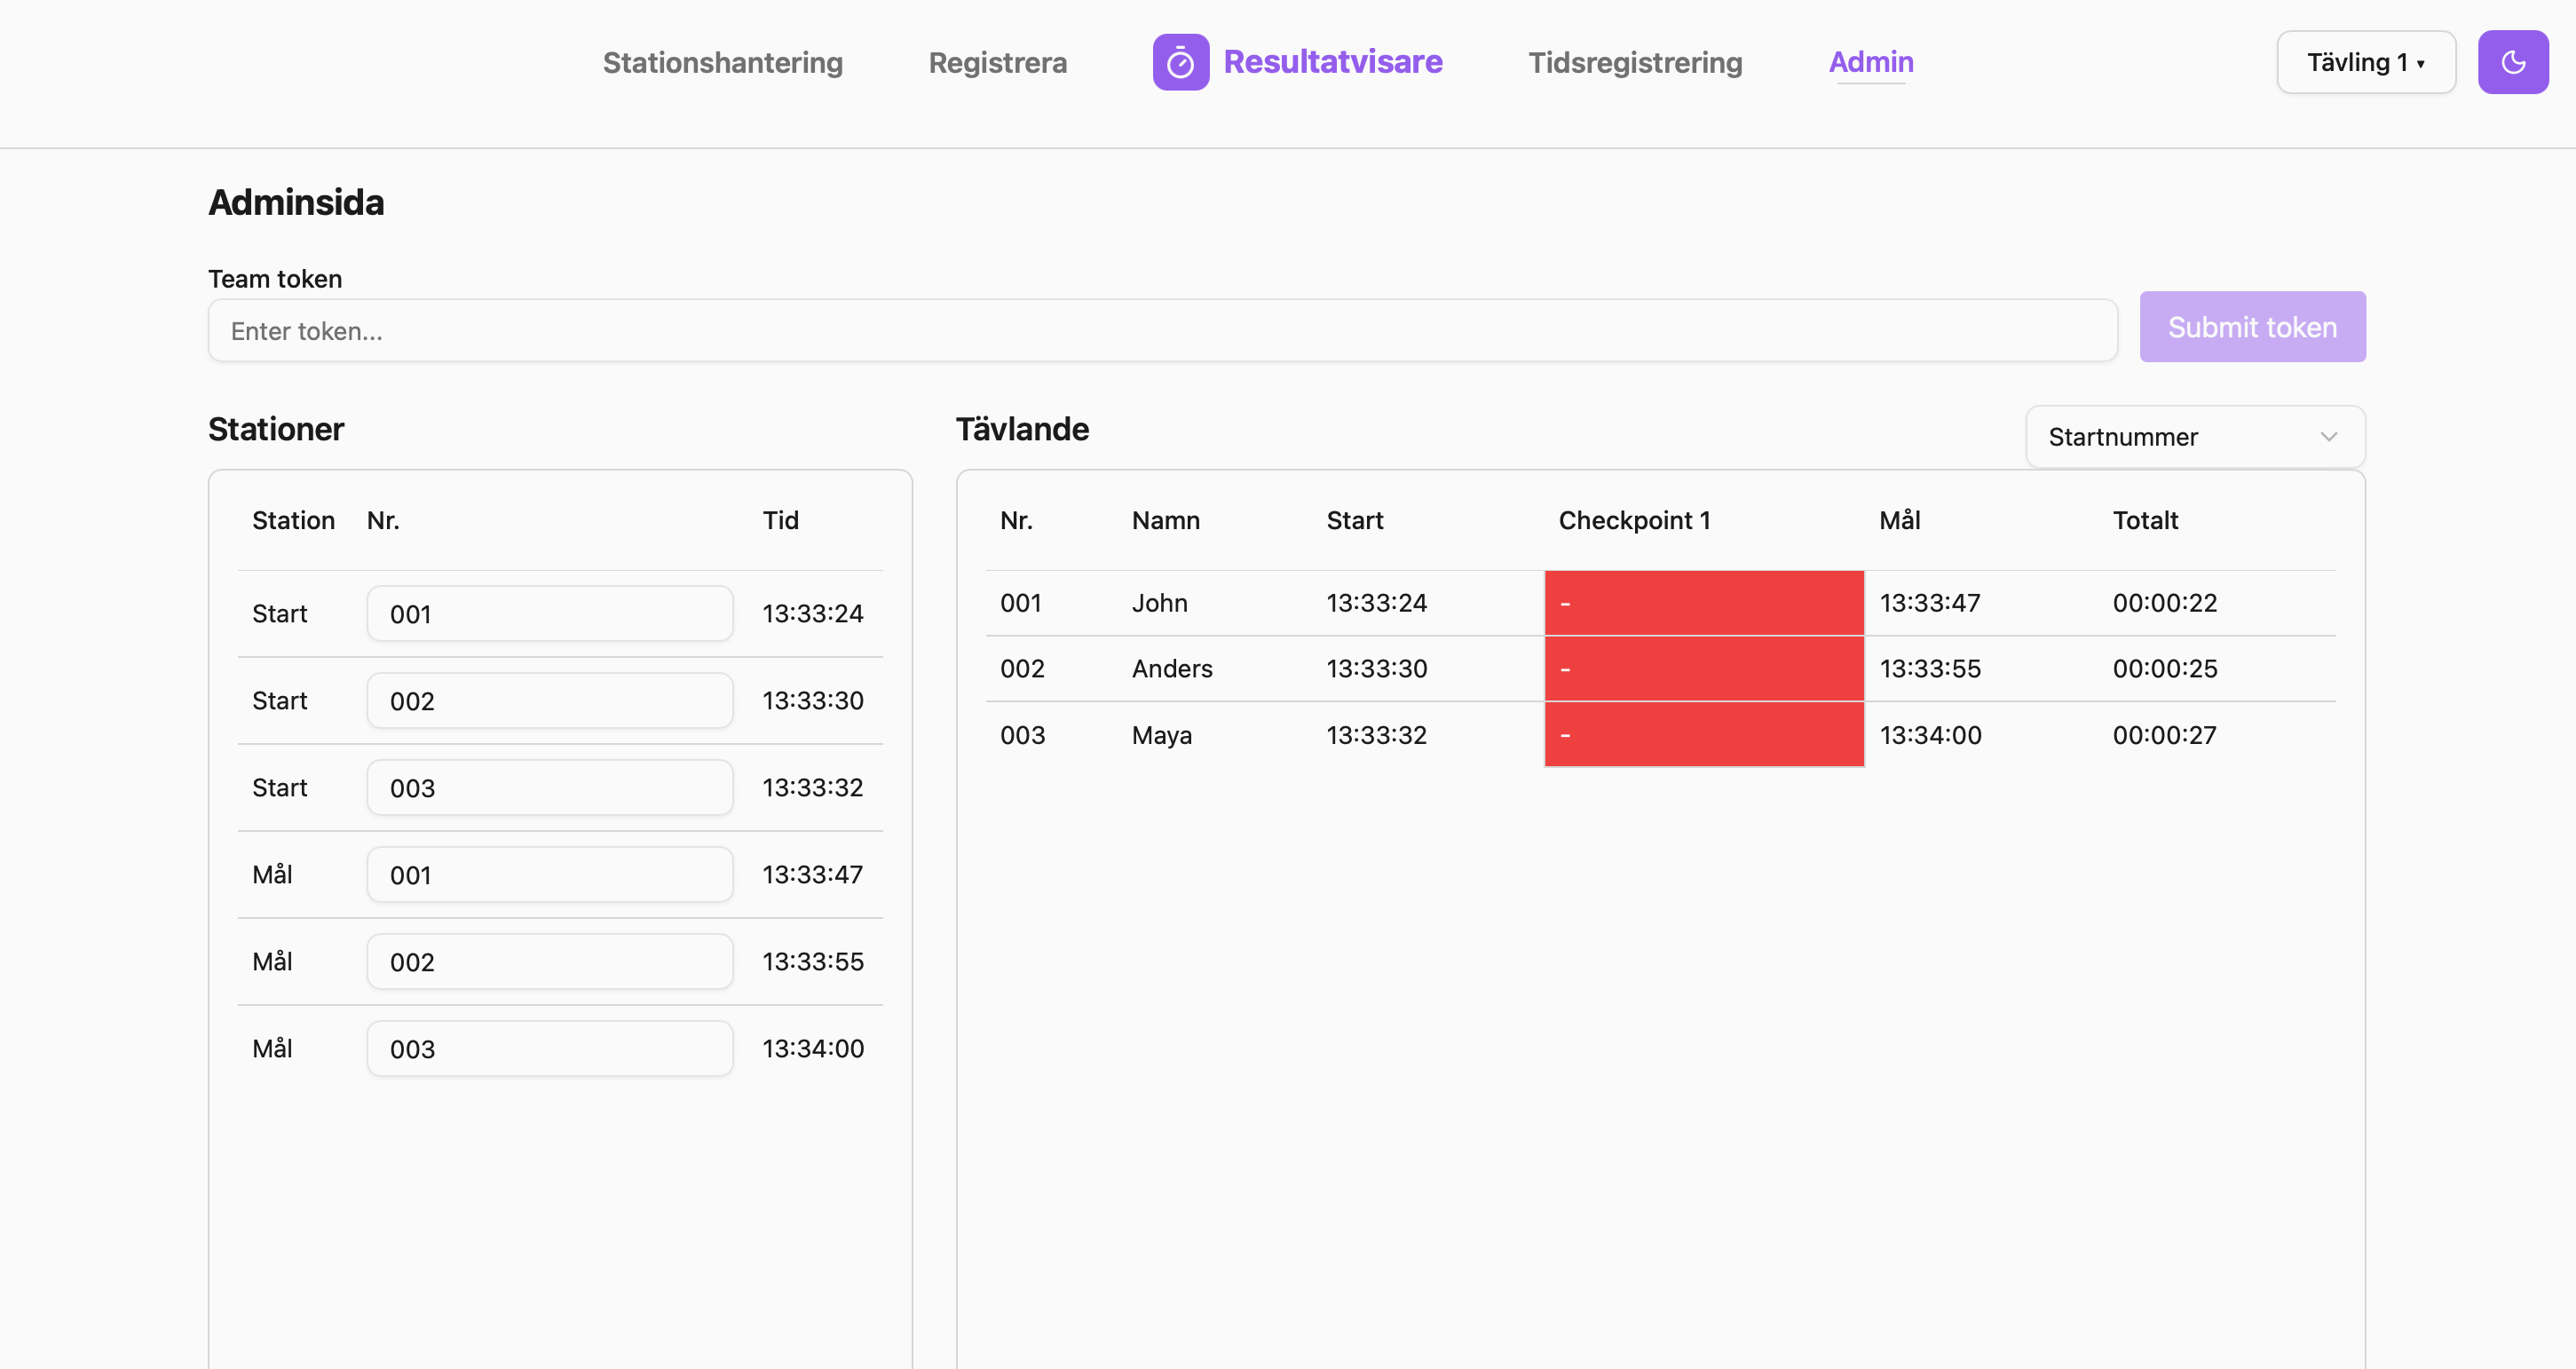
\includegraphics[width=0.7\textwidth]{Screenshots till användarmanual/Admin2.png}
  \caption{Admin-sida}
  \label{fig:Admin}
\end{figure}

\end{document}
